\documentclass[11pt, a4paper, titlepage, openright]{article}

\usepackage{amsmath}
\usepackage[font=small,labelfont=bf]{caption}
\usepackage{float}
\restylefloat{figure}
\usepackage{graphicx}
\usepackage{hyperref}
\usepackage{mathtools}
\usepackage[titletoc, title]{appendix}
\usepackage{listings}
\usepackage{color}
\usepackage{fixltx2e}
\usepackage[bottom]{footmisc}

\usepackage[a4paper, total={6.5in, 9.5in}]{geometry}

\definecolor{dkgreen}{rgb}{0,0.6,0}
\definecolor{gray}{rgb}{0.5,0.5,0.5}
\definecolor{mauve}{rgb}{0.58,0,0.82}

\lstset{frame=tb,
  aboveskip=3mm,
  belowskip=3mm,
  showstringspaces=false,
  columns=flexible,
  basicstyle={\footnotesize\ttfamily},
  numbers=none,
  numberstyle=\tiny\color{gray},
  keywordstyle=\color{blue},
  commentstyle=\color{dkgreen},
  stringstyle=\color{mauve},
  breaklines=true,
  breakatwhitespace=true,
  tabsize=3,
  showstringspaces=false,
  keepspaces=true,
  columns=flexible
  }

\begin{document}
%%%%%%%%%%%%%%%%%%%%%%%%%%%%%%%%%%%%%%%%%
% University Assignment Title Page
% LaTeX Template
% Version 1.0 (27/12/12)
%
% This template has been downloaded from:
% http://www.LaTeXTemplates.com
%
% Original author:
% WikiBooks (http://en.wikibooks.org/wiki/LaTeX/Title_Creation)
%
% License:
% CC BY-NC-SA 3.0 (http://creativecommons.org/licenses/by-nc-sa/3.0/)
%
% Instructions for using this template:
% This title page is capable of being compiled as is. This is not useful for
% including it in another document. To do this, you have two options:
%
% 1) Copy/paste everything between \begin{document} and \end{document}
% starting at \begin{titlepage} and paste this into another LaTeX file where you
% want your title page.
% OR
% 2) Remove everything outside the \begin{titlepage} and \end{titlepage} and
% move this file to the same directory as the LaTeX file you wish to add it to.
% Then add \input{./title_page_1.tex} to your LaTeX file where you want your
% title page.
%
%%%%%%%%%%%%%%%%%%%%%%%%%%%%%%%%%%%%%%%%%

%----------------------------------------------------------------------------------------
%	PACKAGES AND OTHER DOCUMENT CONFIGURATIONS
%----------------------------------------------------------------------------------------
\begin{titlepage}

\newcommand{\HRule}{\rule{\linewidth}{0.5mm}} % Defines a new command for the horizontal lines, change thickness here

\center % Center everything on the page

%----------------------------------------------------------------------------------------
%	HEADING SECTIONS
%----------------------------------------------------------------------------------------

\textsc{\LARGE University of Antwerp}\\[1.5cm] % Name of your university/college
\textsc{\Large }\\[4cm] % Major heading such as course name
\textsc{\Large Scientific Programming}\\[0.5cm] % Minor heading such as course title

%----------------------------------------------------------------------------------------
%	TITLE SECTION
%----------------------------------------------------------------------------------------

\HRule
{ \huge \bfseries Second Session \\ \Large{Exercise 2}}\\ % Title of your document
\HRule \\[1.5cm]

%----------------------------------------------------------------------------------------
%	AUTHOR SECTION
%----------------------------------------------------------------------------------------

\begin{minipage}{0.4\textwidth}
\begin{flushleft} \large
Armin Halilovic - s0122210 % Your name
\end{flushleft}
\end{minipage}
~
\begin{minipage}{0.4\textwidth}
\begin{flushright} \large
\end{flushright}
\end{minipage}\\[4cm]

% If you don't want a supervisor, uncomment the two lines below and remove the section above
%\Large \emph{Author:}\\
%John \textsc{Smith}\\[3cm] % Your name

%----------------------------------------------------------------------------------------
%	DATE SECTION
%----------------------------------------------------------------------------------------

\vfill % Fill the rest of the page with whitespace
{\large August 22, 2016}\\[3cm] % Date, change the \today to a set date if you want to be precise

%----------------------------------------------------------------------------------------
%	LOGO SECTION
%----------------------------------------------------------------------------------------

%\includegraphics{Logo}\\[1cm] % Include a department/university logo - this will require the graphicx package

%----------------------------------------------------------------------------------------


\end{titlepage}
\tableofcontents
\newpage

\section{Problem}
    We are given the function
        \[
            \begin{aligned}
                f(x) = 1 + T_6(x)    && -1 \le x \le 1
            \end{aligned}
        \]
    where \(T_6(x)\) is the Chebyshev polynomial of degree 6.
    We are tasked to calculate the exact integral \[ I = \int_{-1}^1 \! f(x) \, \mathrm{d}x \] using Maple.
    Also, we are tasked to calculate following numerical approximations using Matlab for up to 2 significant numbers:
    \begin{itemize}
        \item The composite trapezoid rule for \( I \)
        \item \( I \) via a Gauss-Legendre integration rule
        \item Monte Carlo integration of  \( I \)
    \end{itemize}

    \begin{figure}[H]
        \begin{minipage}[b]{0.49\textwidth}
            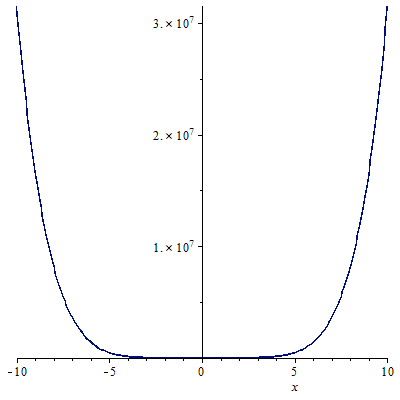
\includegraphics[width=1.0\textwidth]{../maple/mapleChebyPlot.png}
        \end{minipage}
        \hfill
        \begin{minipage}[b]{0.49\textwidth}
            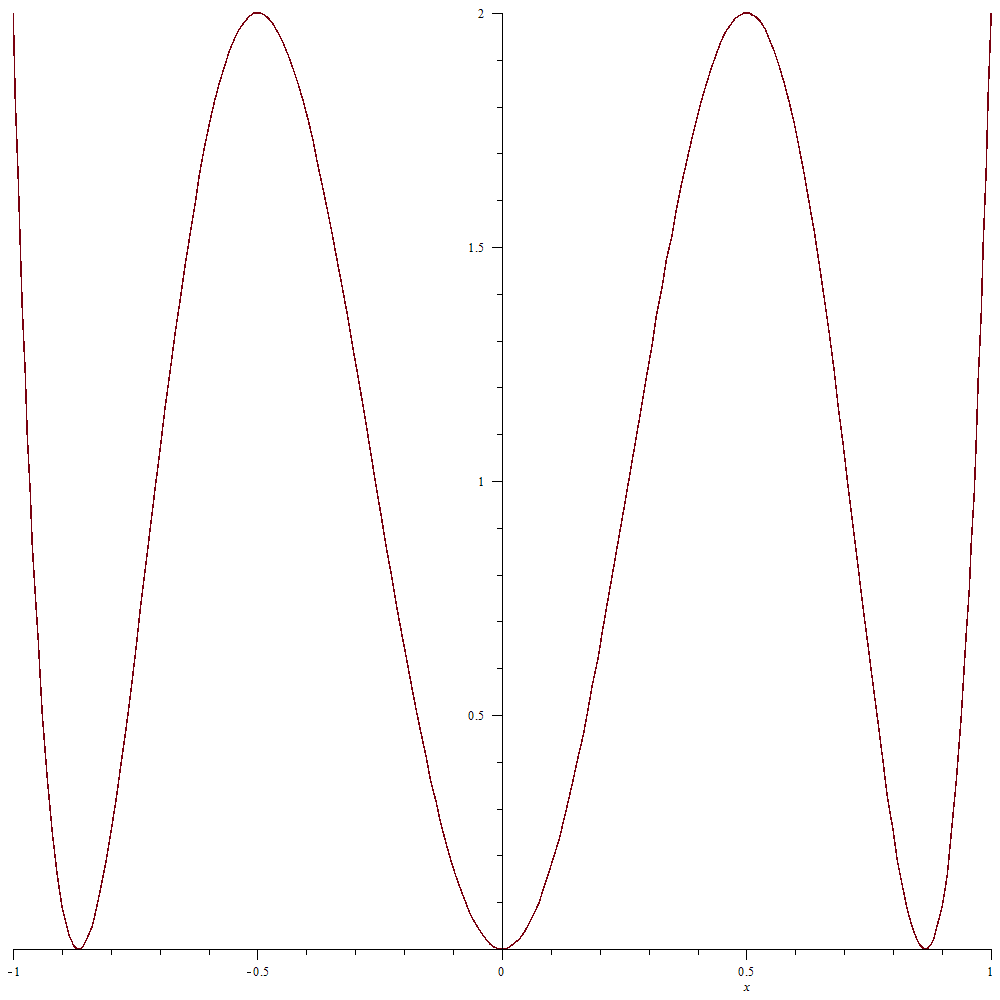
\includegraphics[width=1.0\textwidth]{../maple/mapleChebyPlotZoom.png}
        \end{minipage}
        \caption{Two plots of the given function.}
        \label{fig:function}
    \end{figure}
\bigskip
\bigskip

\section{Using the code}
    All of the Maple and Matlab code can be found under maple/ and matlab/. The matlab code can aslo be found in appendix A.
    The file matlab/solution.m calculates all 3 given tasks and gives the results as output. An example of this output is also included in appendix A.

\newpage

\section{Solutions}
\subsection{Exact calculation}
Using Maple, we find the integral by

\begin{lstlisting}
f := x -> 1 + ChebyshevT(6, x);
int(f(x), x = -1 .. 1);
\end{lstlisting}
and find the result to be
\begin{lstlisting}
68
--
35
\end{lstlisting}
In decimal notation, this is about 1.94.


\subsection{Composite trapezoid rule}
We implement the following function as the composite trapeziodal rule:
\[ I \approx \frac{h}{2} (f(a) + 2 \sum_{i=1}^{n-1} f(x_i) + f(b)) \]
To find the amount of points necessary to achieve the desired precision, we made use of the fact that the error when using this function is bounded by
\[ \frac{5(b-a)^3}{12 N^2} \max_{x \in [a, b]} |f''(x)| \]
If we let
\[ \frac{5(b-a)^3}{12 N^2} \max_{x \in [a, b]} |f''(x)| < 0.1 \]
we find that we need to let n = 119 in the composite trapezoid rule to achieve the desired precision:
\begin{lstlisting}
>> trapeziumN = getCompositeTrapeziumN(@f, -1, 1, 0.1)

trapeziumN =

119

>> compositeTrapeziumArea = eval(compositeTrap2(@(x) f(x), -1, 1, trapeziumN));
>> trapeziumResultAndDifference = [compositeTrapeziumArea  abs(area - compositeTrapeziumArea)]

trapeziumResultAndDifference =

       1.9446    0.0017
\end{lstlisting}


\newpage
\subsection{Gaussian quadrature rules}
To approximate \( I \) via a Gauss-Legendre integration rule, we use the function
\[
 \begin{aligned}
 I \approx \sum_{i=0}^{n} (\frac{b - a}{2}) \ w_i \ f(\frac{a + b}{2} + \frac{(b - a) x_i}{2}) &&&& x_i \in [-1, 1]
 \end{aligned}
 \]
The \(x_i\)'s are the zeroes of the Legendre polynomial of degree n+1.
The weights \( w_i \) are calculated by the function
\[
    w_i = \frac{2}{(1 - x_i^2) * (L_{n+1}'(x_i))^2}
\]
where \( L_i(x) \) is the Legendre polynomial of degree i. \\

To achieve a precision of 2 significant numbers, we need n to equal 3. This means we have only 4 data points, as the
data points are the zeroes of the Legendre polynomial with degree 4.
\begin{lstlisting}
>> gaussLegendreResult = [gaussLegendre(@(x) f(x), -1, 1, 3)]

gaussLegendreResult =

 1.942857142857143
\end{lstlisting}


\subsection{Monte Carlo integration}
To approximate \( I \) via a Monte Carlo integration, we used the general formula
    \[ I \approx (measure\ of\ A) * (average\ of\ f\ over\ n\ random\ points\ in\ A) \]
In our case, the measure of A is the length of the interval we are integrating over: \((1 - -1) = 2\).
Thus, we take \(n\) random points \( x_i \) in the interval \( [-1, 1] \), and then approximate \(I\) by \( 2 * \frac{1}{n} \sum_{i = 1}^{n} f(x_i) \).

Because of the randomness, it is hard to know how many points are necessary to get a precision of
2 significant numbers. We see this in the following example, where n = 200, 500, 1000, 2000, 3500, and 5000.
\begin{lstlisting}
monteCarloResults = [];

for n = [200 500 1000 2000 3500 5000]
    monteCarloArea = monteCarloIntegration(@(x) f(x), -1, 1, n);
    monteCarloResults = [monteCarloResults
                         n monteCarloArea abs(area - monteCarloArea)];
end
monteCarloResults
\end{lstlisting}

\begin{lstlisting}
monteCarloResults =

          200       1.8318      0.11108
          500       1.8744      0.06848
         1000       1.9475    0.0046128
         2000       1.9068     0.036096
         3500       1.9722     0.029297
         5000       1.9223     0.020535
\end{lstlisting}
In this case, we see that 500 points was enough to get a precision of 2 significant numbers,
and that the result was best when n = 1000. We notice that a higher n does not necessarily cause a higher precision.

\onecolumn
\appendix
\appendixpage
\addappheadtotoc

\section{Code}
	\subsection{f.m}
		\lstinputlisting[basicstyle=\scriptsize]{../matlab/f.m}
	\bigskip
	\subsection{compositeTrap2.m}
		\lstinputlisting[basicstyle=\scriptsize]{../matlab/compositeTrap2.m}
	\bigskip
	\subsection{getCompositeTrapeziumN.m}
		\lstinputlisting[basicstyle=\scriptsize]{../matlab/getCompositeTrapeziumN.m}
	\bigskip
	\subsection{gaussLegendre.m}
		\lstinputlisting[basicstyle=\scriptsize]{../matlab/gaussLegendre.m}
	\bigskip
	\subsection{monteCarloIntegration.m}
		\lstinputlisting[basicstyle=\scriptsize]{../matlab/monteCarloIntegration.m}
	\bigskip
	\subsection{solution.m}
		\lstinputlisting[basicstyle=\scriptsize]{../matlab/solution.m}
	\bigskip
\section{Output}
	\subsection{solutionExampleOutput.txt}
		\lstinputlisting[basicstyle=\scriptsize]{../matlab/solutionExampleOutput.txt}
	\bigskip
\newpage
		
\end{document}